%
%

\begin{tikzpicture}[
    font=\small,
    thick,
    mydash/.style={dashed, dash phase=-1.5pt},
    label/.style={align=left, inner sep=0},
    image/.style={inner sep=0, outer sep=0, node distance = 0 and 0}
]
    \pgfplotsset{colormap={warm}{
    rgb=(1, 1, 1)
    rgb=(0.98823499999999997, 0.98039200000000004, 0.87058800000000003)
    rgb=(0.99215699999999996, 0.96470599999999995, 0.71372500000000005)
    rgb=(0.98823499999999997, 0.95686300000000002, 0.64313699999999996)
    rgb=(0.98039200000000004, 0.91764699999999999, 0.50980400000000003)
    rgb=(0.96862700000000002, 0.87451000000000001, 0.40784300000000001)
    rgb=(0.94901999999999997, 0.82352899999999996, 0.32156899999999999)
    rgb=(0.92941200000000002, 0.77647100000000002, 0.27843099999999998)
    rgb=(0.90980399999999995, 0.71764700000000003, 0.235294)
    rgb=(0.89019599999999999, 0.65882399999999997, 0.196078)
    rgb=(0.87843099999999996, 0.61960800000000005, 0.168627)
    rgb=(0.87058800000000003, 0.54901999999999995, 0.156863)
    rgb=(0.85097999999999996, 0.47450999999999999, 0.145098)
    rgb=(0.83137300000000003, 0.41176499999999999, 0.13333300000000001)
    rgb=(0.81176499999999996, 0.34509800000000002, 0.11372500000000001)
    rgb=(0.78823500000000002, 0.26666699999999999, 0.094117599999999996)
    rgb=(0.74117599999999995, 0.18431400000000001, 0.074509800000000001)
    rgb=(0.69019600000000003, 0.12548999999999999, 0.062745099999999998)
    rgb=(0.61960800000000005, 0.062745099999999998, 0.043137300000000003)
    rgb=(0.54901999999999995, 0.027451, 0.070588200000000004)
    rgb=(0.47058800000000001, 0.0156863, 0.090196100000000001)
    rgb=(0.40000000000000002, 0.0039215700000000001, 0.101961)
    rgb=(0.34902, 0, 0.129412)
}}

    % \node[image] (image1)
    % {
    %     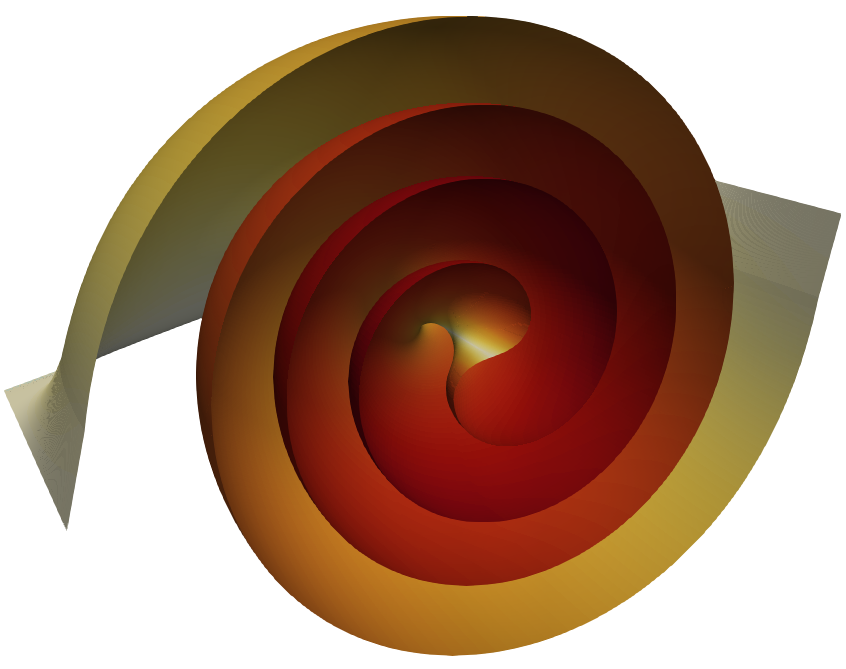
\includegraphics[width=0.5\figurewidth]{figures/ground_truth_log_highres}%
    % };
    % \node[anchor=north] at (image1.south) {\small ground truth};

    \node[image] (image2)
    {
        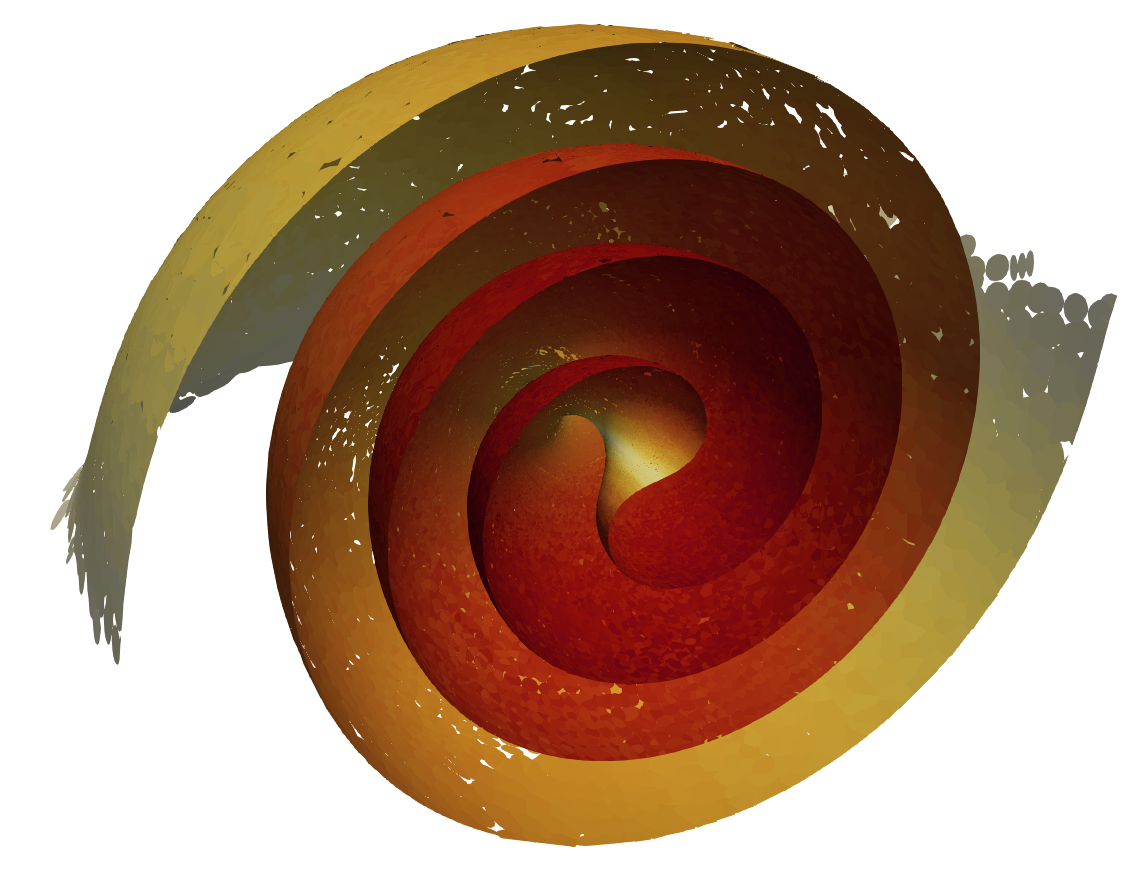
\includegraphics[width=0.5\figurewidth]{figures/norm_0_5_tan_0_01_log}%
    };
    \begin{scope}
        \clip (image2.south) -- (image2.south west) -- (image2.north west) --
            (image2.north);
        \node[image] (gt1) at (image2)
        {
            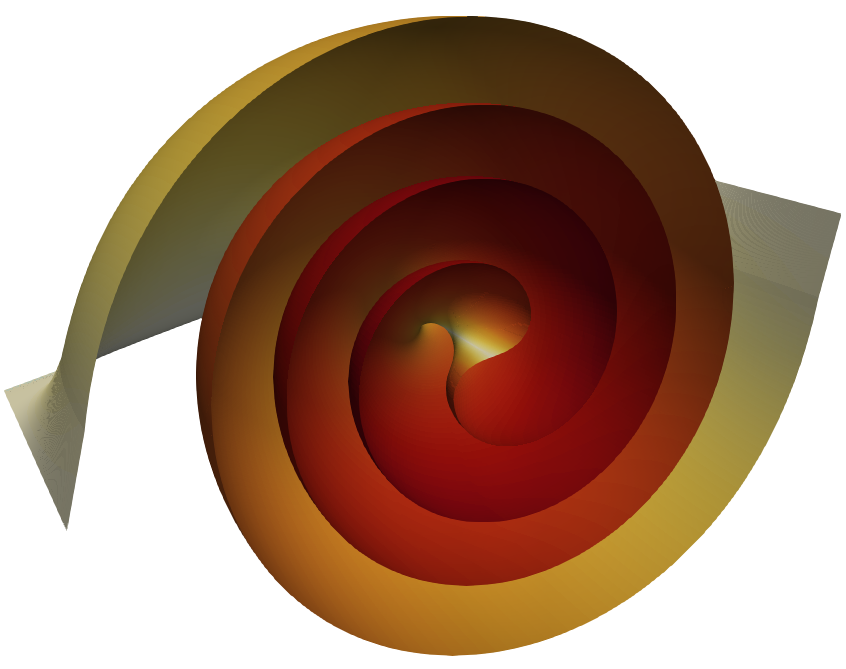
\includegraphics[width=0.5\figurewidth]{figures/ground_truth_log_highres}%
        };
    \end{scope}
    \draw[mydash] (image2.south) -- (image2.north);
    \node[label, anchor=east] at (image2.south east)
    {
        $
        \begin{aligned}
                r_\shortparallel &= 0.01 \\
                N &= \num{143.5}\si{\kilo}
        \end{aligned}
        $
    };
    % \node[label, anchor=south west] at (image2.south west) {ground\\truth};


    \node[image, right=of image2] (image3)
    {
        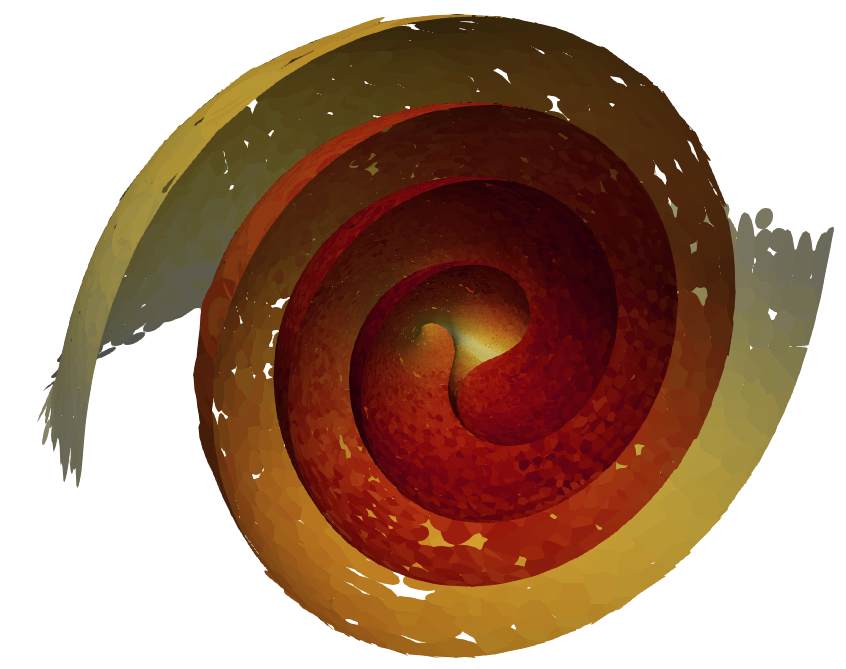
\includegraphics[width=0.5\figurewidth]{figures/norm_0_5_tan_0_02_log}%
    };
    \begin{scope}
        \clip (image3.south) -- (image3.south west) -- (image3.north west) --
            (image3.north);
        \node[image] (gt1) at (image3)
        {
            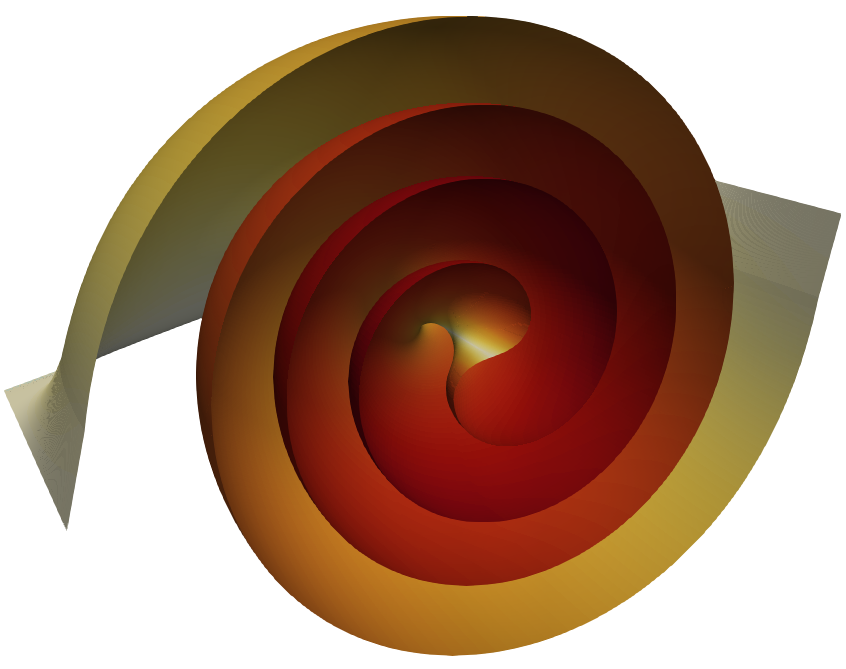
\includegraphics[width=0.5\figurewidth]{figures/ground_truth_log_highres}%
        };
    \end{scope}
    \draw[mydash] (image3.south) -- (image3.north);
    \node[anchor=east] at (image3.south east)
    {
        $
        \begin{aligned}
                r_\shortparallel &= 0.02 \\
                N &= \num{58.1}\si{\kilo}
        \end{aligned}
        $
    };
    % \node[label, anchor=south west] at (image3.south west) {ground\\truth};


    \node[image, below=0.5cm of image2] (image4)
    {
        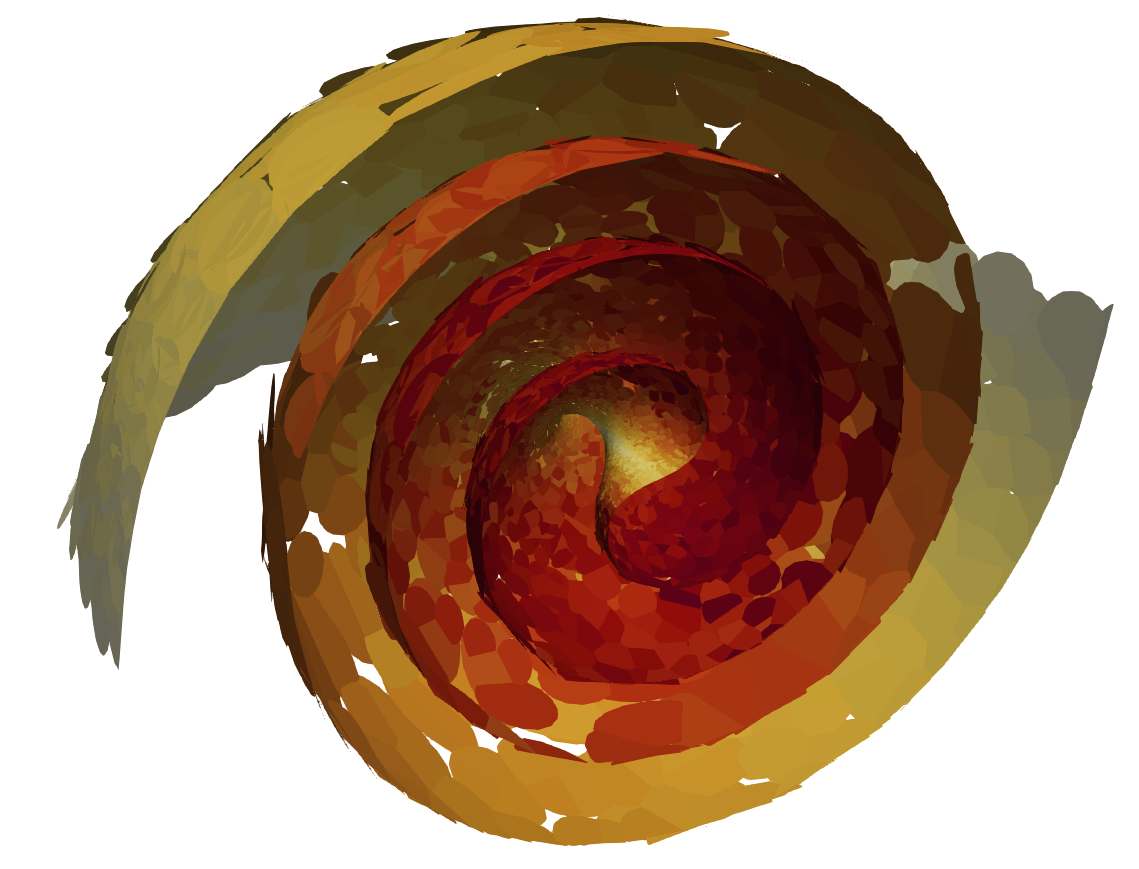
\includegraphics[width=0.5\figurewidth]{figures/norm_0_5_tan_0_05_log}%
    };
    \begin{scope}
        \clip (image4.south) -- (image4.south west) -- (image4.north west) --
            (image4.north);
        \node[image] (gt1) at (image4)
        {
            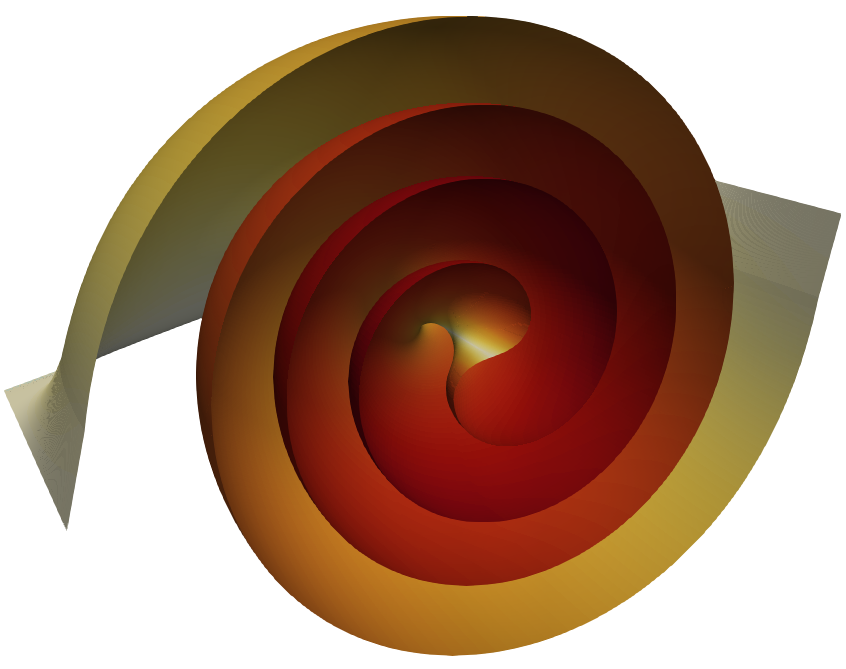
\includegraphics[width=0.5\figurewidth]{figures/ground_truth_log_highres}%
        };
    \end{scope}
    \draw[mydash] (image4.south) -- (image4.north);
    \node[anchor=east] at (image4.south east)
    {
        $
        \begin{aligned}
                r_\shortparallel &= 0.05 \\
                N &= \num{15.4}\si{\kilo}
        \end{aligned}
        $
    };
    % \node[label, anchor=south west] at (image4.south west) {ground\\truth};


    \node[image, right=of image4] (image5)
    {
        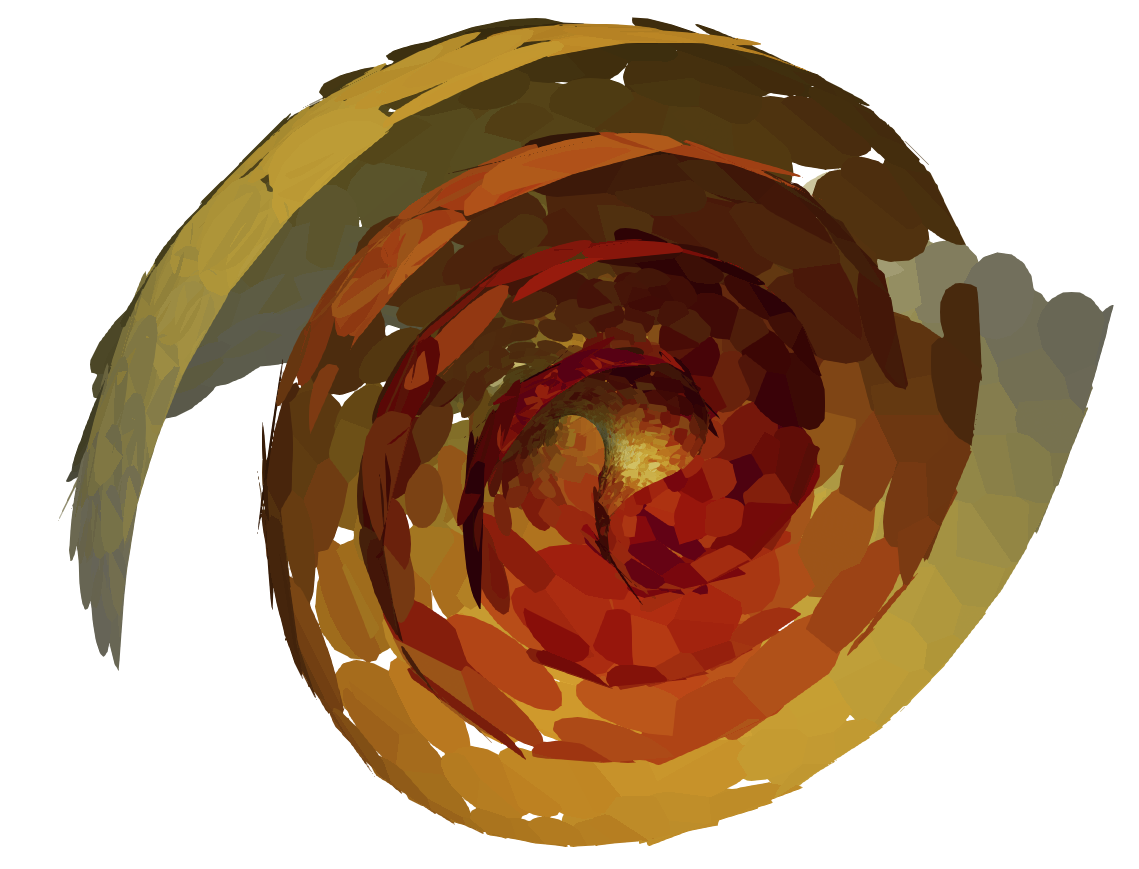
\includegraphics[width=0.5\figurewidth]{figures/norm_0_5_tan_0_1_log}%
    };
    \begin{scope}
        \clip (image5.south) -- (image5.south west) -- (image5.north west) --
            (image5.north);
        \node[image] (gt1) at (image5)
        {
            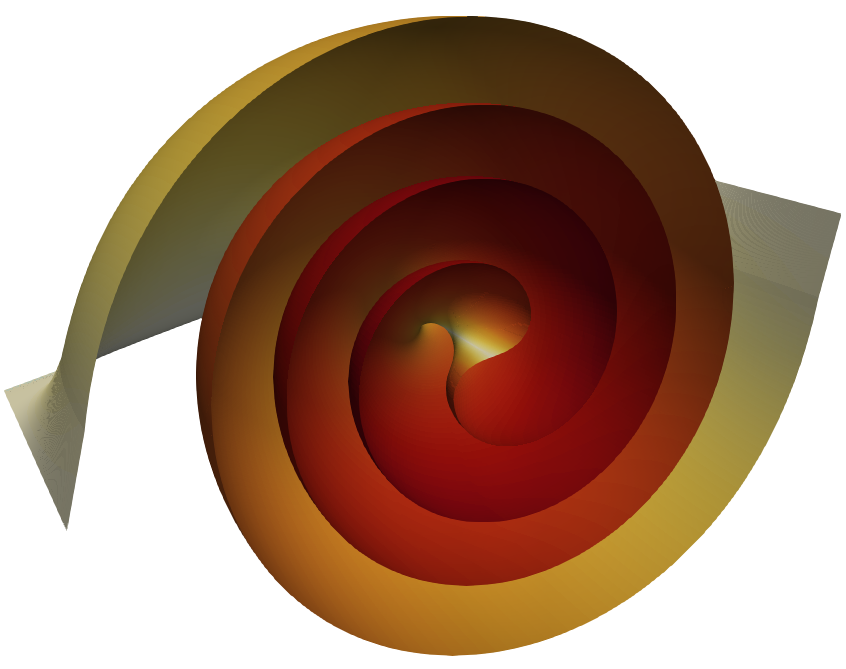
\includegraphics[width=0.5\figurewidth]{figures/ground_truth_log_highres}%
        };
    \end{scope}
    \draw[mydash] (image5.south) -- (image5.north);
    \node[anchor=east] at (image5.south east)
    {
        $
        \begin{aligned}
                r_\shortparallel &= 0.1 \\
                N &= \num{5}\si{\kilo}
        \end{aligned}
        $
    };
    % \node[label, anchor=south west] at (image5.south west) {ground\\truth};


    \node[anchor=north east, yshift=-0.5cm]
        at (image5.south east){
        \begin{axis}[
            scale only axis,
            height=3cm,
            hide axis,
            domain=0:2.1,
            % xmode=log,
            colorbar horizontal,
            colorbar/width=0.25cm,
            colormap name={warm},
            point meta min=0, point meta max=2.1,
            colorbar style={
                title=$c$,
                scaled ticks=false,
                % xmode=log,
                xtick={0, 1, 2},
                xticklabels = {$10^{\,0}$, $10^{\,1}$, $10^{\,2}$}
            }]
          \end{axis}
    };

\end{tikzpicture}